\section{Evolutionary Test in Load, Performance and Stress Tests}

The search for the longest execution time is regarded as a discontinuous, nonlinear, optimization problem, with the input domain of the system under test as search space \cite{Sullivan}. The main objective of evolutionary testing in performance,stress and load tests is to find test scenarios which produce execution times violating the timing constraints specified. If a temporal error is found, the test was successful \cite{Sullivan}. The application of evolutionary algorithms to load, performance and stress tests involves finding the best and worst case execution times (BCET, WCET) to determine if timing constraints are fulfilled \cite{Afzal2009a}. 

Evolutionary tests uses a cost (fitnesse) function to select the best individuals. There has two measurement units normally associated with the fitnesse function in load, performance or stress test: Processor Cycles and Execution Time. The Processor Cycles approach describes a fitness function in terms of processor cycles. The Execution Time approach involves executing the application under test measuring the execution time \cite{Afzal2009} \cite{tracey2000search}.
% * <naubergois@gmail.com> 2015-09-17T01:17:52.488Z:
%
%  Rever esse paragrafo
%
The Figure \ref{fig:comparison}  shows a comparison between the presented research work and the load, performance and stress test researches presented by Afzal et. al. \cite{Afzal2009}. Afzal's work was added with some of the latest research in the area (\cite{Garousi2006} \cite{Garousi2010}). The x axis represents the type of tool used ( Prototype or Functional Tool )  and the y axis presents the metaheuristic used by each research (Genetic Algorithm, Tabu Search, Simulated Annnealing or a Customized Algorithm). The Figure also divides the researches by the type of function fitnesse (Execution Time or Processor Cycles). Most research is limited to making prototypes on genetic algorithms. The presented research work is distinguished from others by having a functional tool using a hybrid approach. 

% * <naubergois@gmail.com> 2015-09-17T01:22:09.554Z:
%
%  Customized Algorithm
%

\begin{figure}[h]
\centering
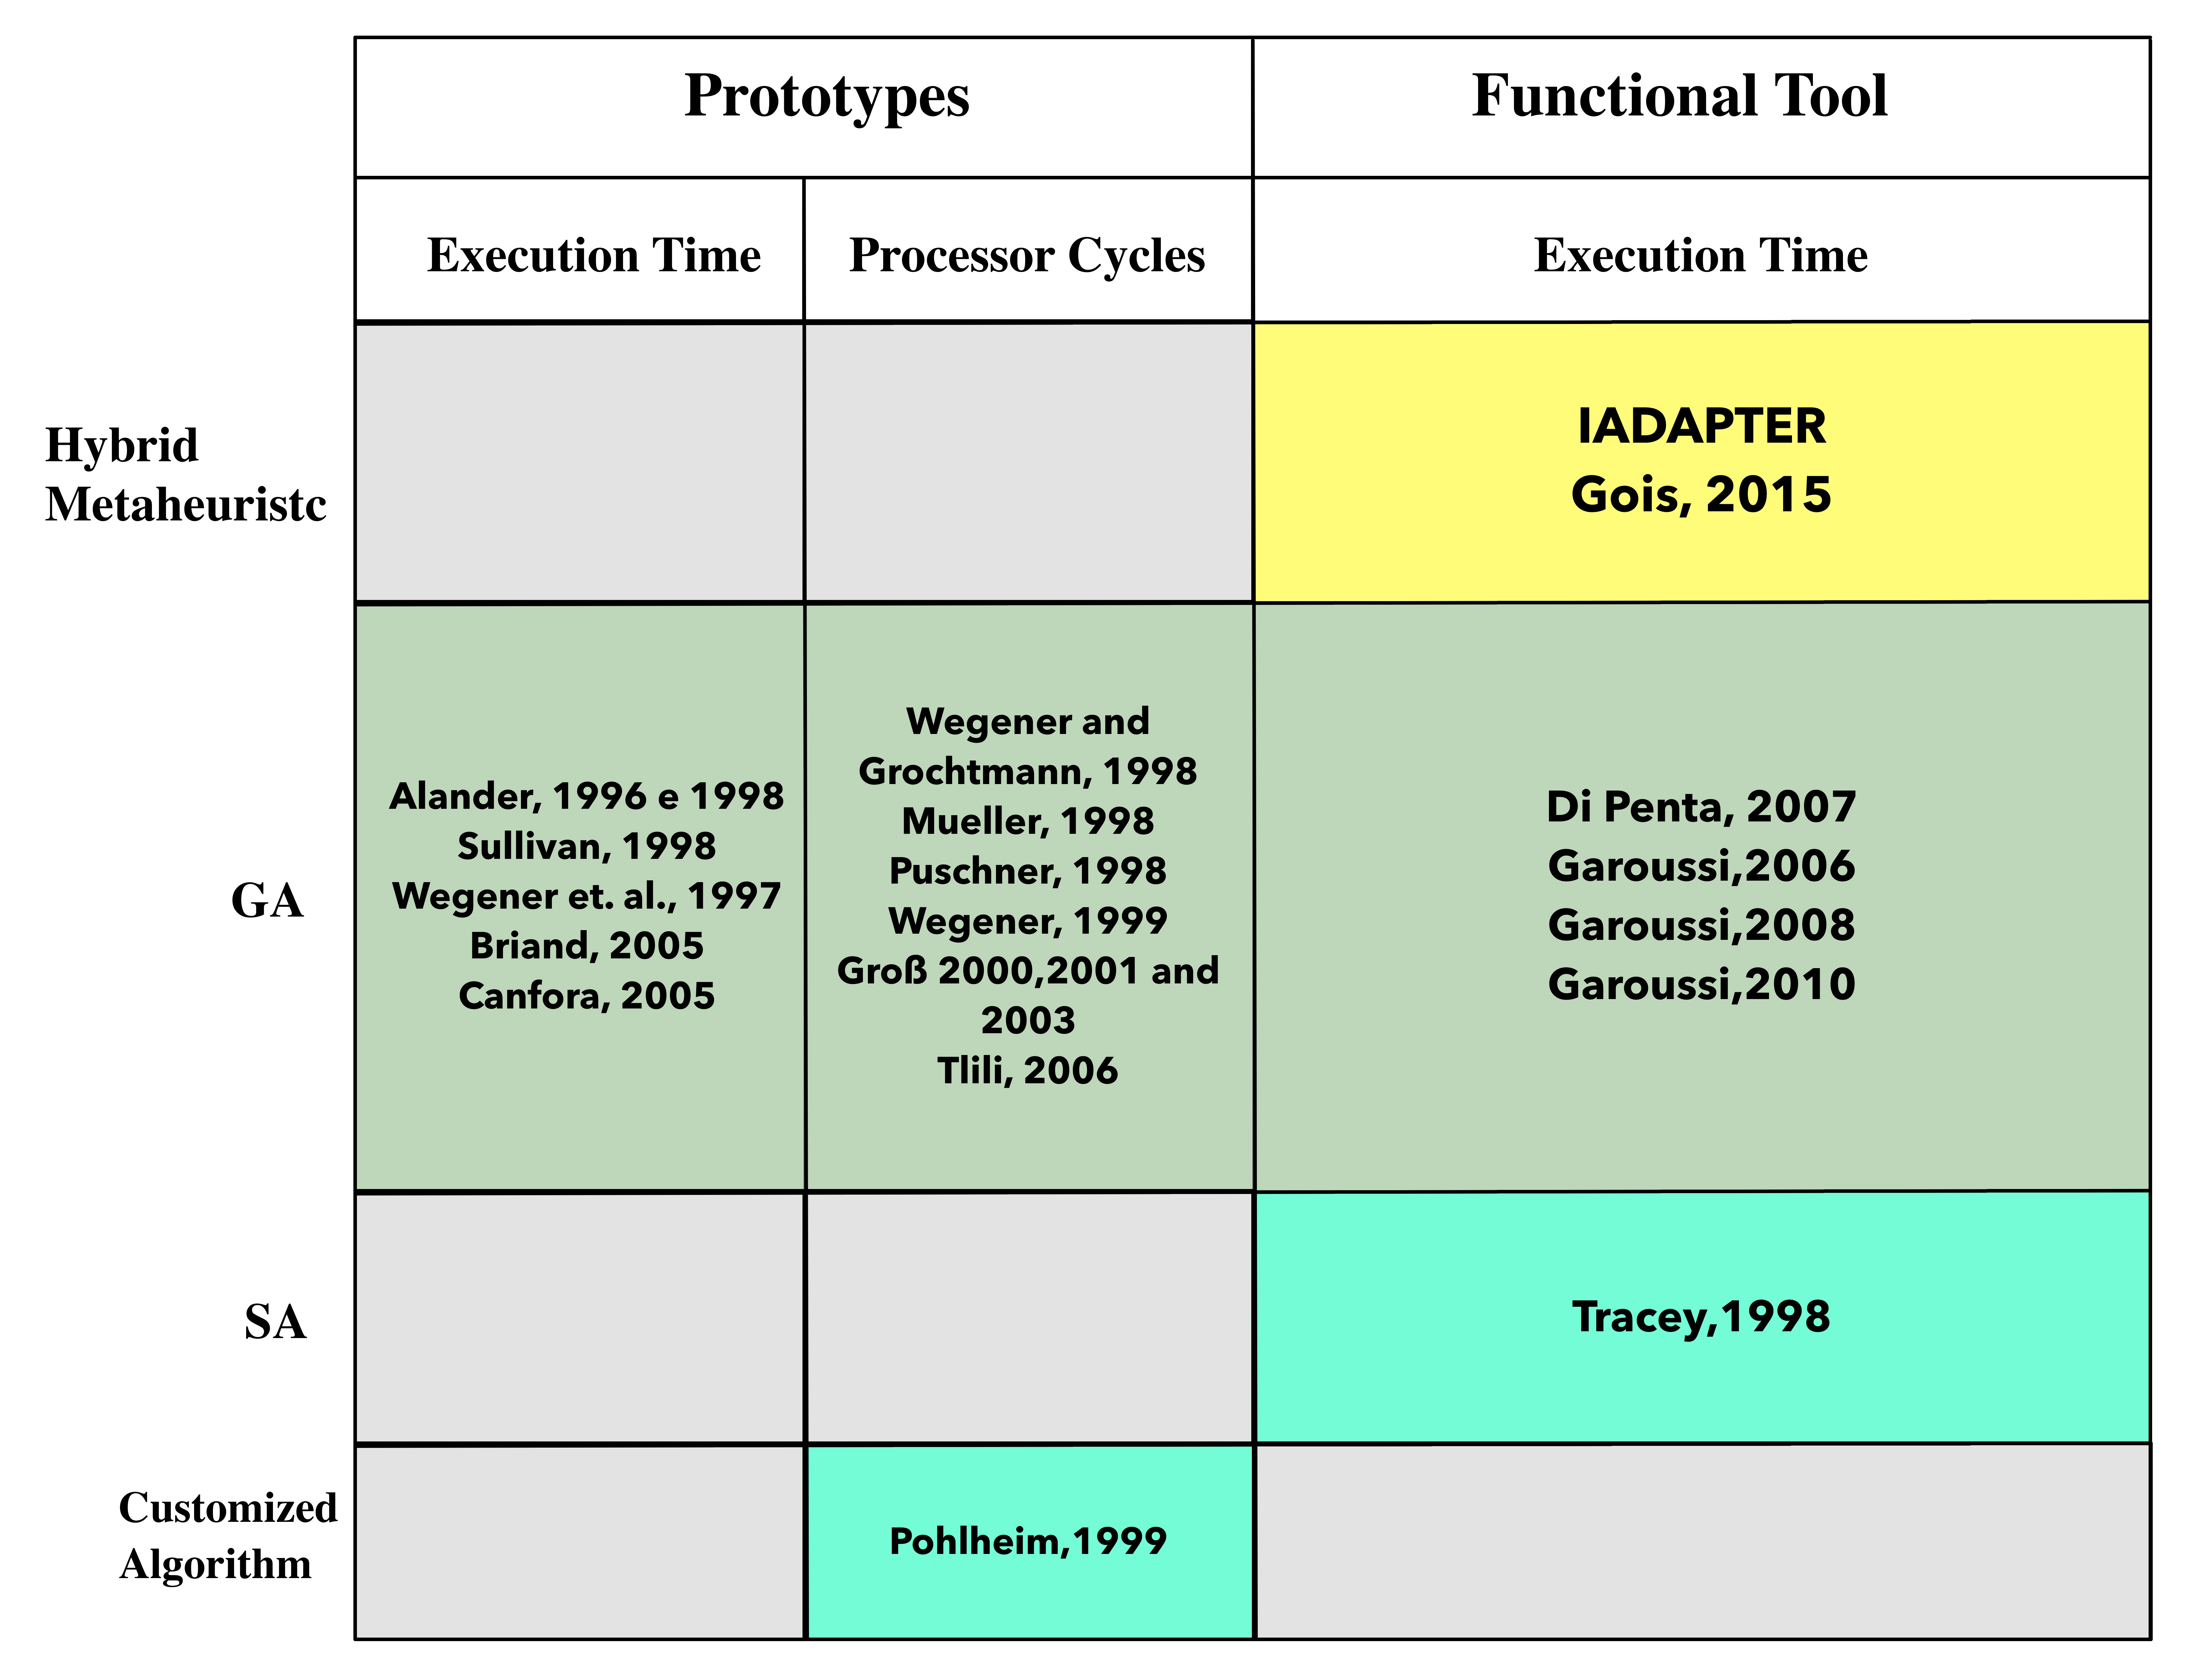
\includegraphics[width=0.5\textwidth]{./images/comparativo1.png}
\caption{
Distribution of the researches over range of applied metaheuristics}
\label{fig:comparison}
\end{figure}